\documentclass{article}

\usepackage[utf8]{inputenc}
\usepackage[frenchb]{babel}

\usepackage{hyperref}
\usepackage{graphicx}

\usepackage{listings}
\lstdefinestyle{customstyle}{
    basicstyle=\footnotesize,
    breakatwhitespace=false,         
    breaklines=true,                 
    captionpos=b,                    
    keepspaces=true,                                                                                       
    tabsize=4,
    frame=single, %lines
    moredelim=[is][\underbar]{_}{_} % underlines permitted without escape character
}
\lstset{style=customstyle}

\title{Free Basic to C compiler}
\author{Jérémy Bardon}

\begin{document}
	\maketitle

\section{Introduction}
Le but de ce projet est de créer un compilateur capable de convertir un code écrit 
en \href{http://www.freebasic.net}{Free Basic} dans le langage C. 

\begin{figure}[h]
    \centering
    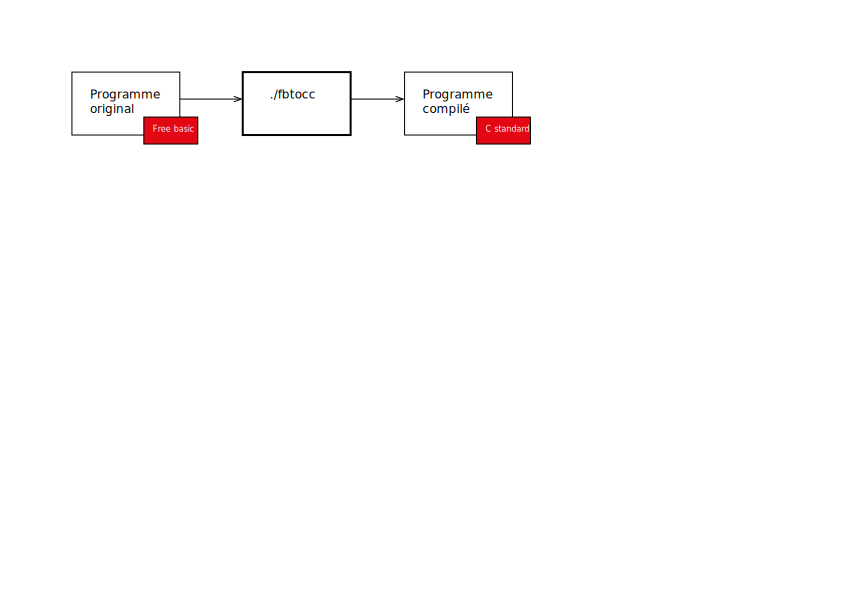
\includegraphics[scale=0.6]{schema.png}
    \caption{Rôle du compilateur}
\end{figure}
	
Le programme en C
ainsi généré sera compilable avec \emph{gcc} et effectuera les mêmes opérations que 
le programme original.
	
\section{Adaptations}
Par défaut, un programme écrit en free basic dispose comme en C d'un 
certain nombre de fonctions que l'on peut utiliser sans inclure des programmes 
externes. Cependant, ces fonctions \og{}basiques\fg{} ne sont pas équivalentes dans 
les deux langages.
\\\\
L'exemple le plus simple est la fonction qui permet d'afficher un message : en 
free basic il s'agit de la fonction \emph{print} qui est incluse 
par défaut mais en C il est nécessaire d'inclure \emph{stdio.h}.
\\\\
Une autre différence de taille est la présence -- en C -- d'une routine principale 
(main) qui doit être présente dans tout programme écrit en C. Ce n'est pas le cas du 
free basic qui propose une structure plus libre du programme.

\lstset{language=c,caption=Programme C englobant}
\lstinputlisting{wrap.c}

Ce sont ces différences qui amènent à devoir proposer une structure englobante d'un 
programme dans laquelle on va ensuite insérer le code free basic converti.
	
\section{Grammaire}
\begin{itemize}
\item Fonction à 1 argument (affichage d'un message)
\item Déclaration de constantes (entier et chaîne de caractères)
\item Déclaration et changement de valeur de variables (entier et chaîne de caractères)
\item Commentaire mono-ligne
\item Condition simple (pas de close sinon)
\item Report du numéro de ligne et de caractère en cas d'erreur lors du parsing
\end{itemize}
	
\section{Reconnaissance des erreurs}
Dans sa première version -- qui est l'actuelle version --, le compilateur ne gère pas 
les erreurs de logique dans le code en free basic mais seulement les défauts d'ordre
syntaxiques.
\\\\
On fait donc l'hypothèse que le code en entrée est compilable et exécutable sans erreurs
ce qui permet de se concentrer d'avantage sur la reconnaissance -- et la conversion -- 
de nombreux éléments du langage.
\\\\
L'architecture interne du compilateur -- décrite plus bas -- a été pensée pour permettre
l'intégration de cette fonctionnalité. En effet, tout les éléments sont stockés sous forme
d'un arbre syntaxique et les variables sont sauvegardées dans un registre.	
	
\section{Fonctionnement interne}
Au delà de l'analyse lexicale plutôt générique, la partie intéressante se situe au niveau
de l'analyse syntaxique. En effet, lors de cette phase on vérifie pas le sens que avoir 
une ligne de code mais 
seulement si elle est bien organisé. 
\\\\
Le compilateur ne se contente pas transformer 
chaque ligne en une autre sous forme des chaine de caractères mais il construit un 
arbre syntaxique qui permet d'identifier clairement comment s'enchainent les instructions
et quel sont leur sens (définition de variable, condition, boucle..).
\\\\
En parallèle de cet arbre, il tient à jour un registre des variables -- sous forme de 
table de hashage -- qui sont déclarés dans le programme afin de pouvoir afficher 
différemment un entier et une chaine de caractères. Ce registre retient donc le nom et le
type de chaque variable ce qui rend facilement possible la traduction d'une comparaison 
entres des entiers ou entre des chaines de caractères.
\\\\
Une fois l'arbre construit et le registre rempli, un algorithme parcours l'arbre et 
s'occupe de transformer chaque élément sous forme de chaîne de caractère correspondant
à un code C valide.

\end{document}